\documentclass{article}
\usepackage[utf8]{inputenc}
\usepackage{amsmath}
\usepackage{graphicx}
\usepackage{BeginnerStyleFile}
\usepackage{scrextend}
\graphicspath{ {images/} }

\title{Reading Summary 1.3}
\author{Evan Hughes}
\date{January 2023}

\begin{document}
\maketitle
\section*{Prime and Unique Factorization}
Every nonzero integer $n$ except $\pm 1$ has at least four distinct
divisors, namely $1, -1, n, -n$. Integers that have only these four divisors play a crucial role.

\textbf{Definition}
\begin{center}
    An integer $p$ is said to be prime if $p \neq 0, \pm 1$ and
    the only divisors of $p$ are $\pm1$ and $\pm p$.
\end{center}

\textbf{Example:}( from the book) 

$3, 5, 7, 11, 13, 17$ are prime, but $15$ is not (because 15 has divisors other than $\pm 1$ and $\pm 15$).
The integer 4567 is prime, but proving this fact from the definitions requires a tedious check of all its possible divisors.
Fortunately, there are more efficient methods for determining
whether an integer is prime.
\vspace{5mm}

It is not difficult to show that there are infinitely many distinct primes.
Because an integer $p$ has the same divisors as $-p$, we see that
\begin{center}
    $p$ is prime if and only if $-p$ is prime.
\end{center}
If $p$ and $q$ are both prime and $p\mid q$, then $p$ must be one of $1, -1, q, -q$.
But since $p$ is prime, $p \neq \pm 1$. Hence,
\begin{center}
    if $p$ and $q$ are both prime and $p \mid q$, then $p = \pm q$.
\end{center}

\subsection*{Theorem 1.5}
Let $p$ be an integer with $p \neq 0, \pm 1$. Then $p$ is prime if and only if $p$ has this property:
\begin{center}
    If $p \mid bc$, then $p \mid b$ or $p \mid c$.
\end{center}

\subsection*{Corollary 1.6}
If $p$ is prime and $p \mid a_1 a_2 \ldots a_n$, then $p$ divides at least one $a_i$.

If you factor any integer other than $0$ or $\pm1$, ``as much as possible'', it will be a product of one or more primes

\textbf{Example:} $4598 = 2^1 * 11^2 * 19^1$

\subsection*{Theorem 1.7}
Every integer $n$ other than $0$ and $\pm 1$ is a product of primes.

\subsection*{Theorem 1.8 (Fundamental Theorem of Arithmetic)}
Every integer $n$ other than $0$ and $\pm 1$ is a product of primes. This prime factorization is
unique in the following sense: if
\begin{center}
    $n = p_1p_2\cdots p_r$ and $n = q_1q_2\cdots q_s$
\end{center}
with each $p_r$, $q_r$ prime, then $r = s$(number of factors are the same) and
\begin{center}
    $p_1 = \pm q_1, p_2 = \pm q_2, \ldots, p_r = \pm q_s$.
\end{center}
\begin{figure}[h]
    \centering
    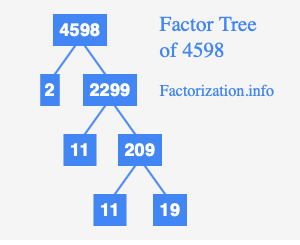
\includegraphics[scale=0.7]{factor-tree-of-4598.png}
    \caption{Factor Tree of 4598}\label{fig:Factor Tree of 4598}
\end{figure}

\subsection*{Corollary 1.9}
Every integer $n > 1$ can be written in one and only one way in the form of 
$n = p_1p_2\cdots p_n$ where $p_i$ are positive primes with 
$p_1 \leq p_2 \leq \cdots \leq p_n$.

\subsection*{Theorem 1.10}
Let $n > 1$, if $n$ has no positive prime factor less than or equal to $\sqrt{n}$,
then $n$ is prime.
\end{document}